\chapter{Projection-Based Evaluation of Tukey Depth from Weighted Student Differences}

\section{Definition and Notation}

In \cite{Ruben1960}, the distribution of a weighted difference of two independent Student variables is derived in the univariate setting (\(d=1\)). For a given angle \(\theta\) and independent Student variables \(t_1\) and \(t_2\) with degrees of freedom \(\nu_1\) and \(\nu_2\), respectively, one considers the random variable
\[
v = t_1\sin\theta - t_2\cos\theta.
\]
Although the original derivation employs the difference, the substitution of a plus sign is justified by the symmetry of the Student distribution. Moreover, this modification allows the extension of the range of \(\theta\) from the usual \([0,\pi/2]\) to the full circle \([0,2\pi)\) without affecting the final density.

Following the approach in \cite{Ruben1960}, the cumulative distribution function (CDF) of \(v\) is given by
\[
F_v(v_0)=\int_0^1 \Pr\Bigl\{T_{\nu_1+\nu_2}\le v_0\,\varphi(u)\Bigr\}\,\frac{u^{\nu_1/2-1}(1-u)^{\nu_2/2-1}}{B(\nu_1/2,\nu_2/2)}\,du,
\]
where
\[
\varphi(u)=\sqrt{\frac{\sin^2\theta}{u}+\frac{\cos^2\theta}{1-u}},
\]
and \(T_{\nu_1+\nu_2}\) denotes a Student variable with \(\nu_1+\nu_2\) degrees of freedom. Note that the squared trigonometric terms eliminate any sign ambiguity, ensuring the expression remains valid for any \(\theta\in[0,2\pi)\).

\section{The Projection Method and Computation of Tukey Depth}

In the multivariate setting, the classical definition of the Tukey (halfspace) depth of a point \(x\in\mathbb{R}^p\) with respect to a probability measure \(F\) is given by
\[
\mathrm{TD}(x)=\inf_{u\in S^{p-1}} F\Bigl(\{y\in\mathbb{R}^p:\langle y,u\rangle\ge \langle x,u\rangle\}\Bigr),
\]
i.e. the smallest probability mass in any closed halfspace that contains \(x\).

Our investigation begins by studying the distribution of the weighted sum
\[
v = t_1\sin\theta + t_2\cos\theta,
\]
whose CDF is expressed as
\[
F_v(v_0)=\int_0^1 \Pr\Bigl\{T_{\nu_1+\nu_2}\le v_0\,\varphi(u)\Bigr\}\,\frac{u^{\nu_1/2-1}(1-u)^{\nu_2/2-1}}{B(\nu_1/2,\nu_2/2)}\,du,
\]
with
\[
\varphi(u)=\sqrt{\frac{\sin^2\theta}{u}+\frac{\cos^2\theta}{1-u}},
\]
and where \(T_{\nu_1+\nu_2}\) is a Student variable with \(\nu_1+\nu_2\) degrees of freedom. Notice that by considering the complementary probability \(1-F_v(v_0)\), we obtain the mass contained in the halfspace corresponding to the projection direction determined by \(\theta\).

To connect this univariate result to the multivariate Tukey depth, note that if we were to compute the depth by considering all possible projection directions, we would have
\[
\mathrm{TD}(x)=\inf_{\theta\in[0,2\pi)} \{1-F_v(v_0(\theta))\},
\]
where \(v_0(\theta)\) denotes the threshold in the projected one-dimensional space corresponding to the halfspace boundary for direction \(\theta\).

Under the assumption of elliptical symmetry, it can be shown that the infimum is achieved when the projection is aligned with the point \(x\). That is, by choosing the optimal projection direction
\[
u=\frac{x}{\|x\|},
\]
the scalar projection of \(x\) becomes exactly \(\|x\|\). Hence, the Tukey depth simplifies to
\[
\mathrm{TD}(x)=1-F_v\bigl(\|x\|\bigr)=1-\mathbb{E}\Bigl[G\Bigl(\|x\|\,\varphi(U)\Bigr)\Bigr],
\]
where
\[
G(t)=\Pr\{T_{\nu_1+\nu_2}\le t\},
\]
and \(U\) is a Beta random variable with density
\[
f_U(u)=\frac{u^{\nu_1/2-1}(1-u)^{\nu_2/2-1}}{B(\nu_1/2,\nu_2/2)}.
\]
This formulation connects our analysis of the weighted sum \(v\) to the classical Tukey depth definition by demonstrating that, under optimal projection, the centrality of \(x\) is measured by the probability mass in the halfspace determined by \(x/\|x\|\). Consequently, the computation of \(\mathrm{TD}(x)\) reduces to evaluating a univariate expectation.

\section{Numerical Evaluation and Monte Carlo Approximation}

The integral representation of \(F_v(v_0)\) can be recast in expectation form. Define
\[
G(t)=\Pr\{T_{\nu_1+\nu_2}\le t\},
\]
and let \(U\) be a Beta random variable with density
\[
f_U(u)=\frac{u^{\nu_1/2-1}(1-u)^{\nu_2/2-1}}{B(\nu_1/2,\nu_2/2)}, \quad 0\le u\le 1.
\]
Then the CDF can be written as
\[
F_v(v_0)=\mathbb{E}\Bigl[G\bigl(v_0\,\varphi(U)\bigr)\Bigr].
\]
In practice, this one-dimensional integral is computed either by numerical quadrature or by Monte Carlo simulation. In the quadrature approach, one employs standard routines to evaluate
\[
\int_0^1 G\Bigl(v_0\,\varphi(u)\Bigr)f_U(u)\,du,
\]
while in a Monte Carlo approximation one would generate \(N\) independent samples \(u_1,\ldots,u_N\) from the Beta distribution and approximate the expectation by
\[
\widehat{F_v}(v_0)=\frac{1}{N}\sum_{i=1}^N G\Bigl(v_0\,\varphi(u_i)\Bigr).
\]
This reduction to a one-dimensional expectation is particularly attractive in view of its computational tractability.

\section{Visualization}

For the purpose of illustration, we now specialize to the case where \(\nu_1=\nu_2=v\). Under this simplification, the density of \(U\) becomes
\[
f_U(u)=\frac{u^{v/2-1}(1-u)^{v/2-1}}{B(v/2,v/2)},
\]
and the depth formula reduces to
\[
\mathrm{TD}(x)=1-\int_0^1 G\Bigl(\|x\|\,\varphi(u)\Bigr)f_U(u)\,du,
\]
with the optimal projection determined by \(x/\|x\|\).

To provide a concrete visual interpretation, consider contour plots of the Tukey depth in \(\mathbb{R}^2\). In these plots, the depth at a point \(x\) is computed as above, with the scalar projection given by its Euclidean norm. Figure~\ref{fig:TD_contour} shows three panels corresponding to different values of the degrees-of-freedom parameter \(v\): \(v=1\), \(v=5\), and \(v=100\). In each case the depth is calculated over a grid of points, and the contour plots illustrate how the depth function changes with \(v\) and provide insight into the centrality of points in the plane as measured by Tukey depth.

\begin{figure}[htbp]
  \centering
  
  % First image
  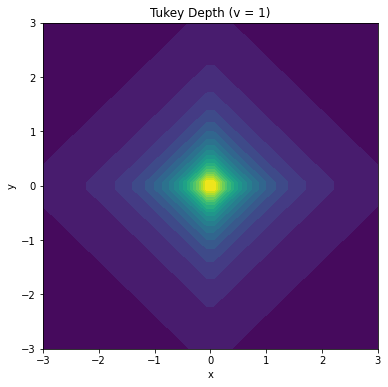
\includegraphics[width=0.3\textwidth]{images/TD_v1.png}
  \hspace{1em}
  % Second image
  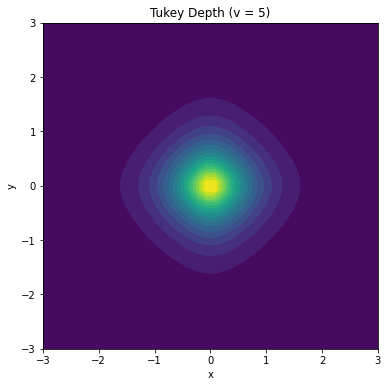
\includegraphics[width=0.3\textwidth]{images/TD_v5.png}
  \hspace{1em}
  % Third image
  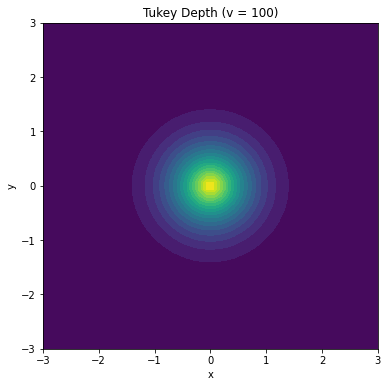
\includegraphics[width=0.3\textwidth]{images/TD_v100.png}
  
  \caption{Contour plots of the Tukey Depth for three values of \(v\).}
  \label{fig:TD_contour}
\end{figure}